\documentclass{article}
	\usepackage{geometry}
	\geometry{left=1.0cm,right=1.0cm}
	\usepackage{graphicx}
	\usepackage{indentfirst}
	\usepackage[hyphens]{url}
	\usepackage{listings}
	\usepackage{color}
	\definecolor{gray}{rgb}{0.3,0.3,0.3}
	\usepackage{caption}
	\DeclareCaptionFont{white}{\color{white}}
	\DeclareCaptionFormat{listing}{\colorbox{gray}{\parbox{\textwidth}{#1#2#3}}}
	\captionsetup[lstlisting]{format=listing,labelfont={bf,sf,white},textfont={bf,sf,white}}
	\usepackage{xcolor}
	\usepackage{booktabs}
	\captionsetup[table]{labelfont=bf}
	\usepackage[colorlinks,linkcolor=red]{hyperref}

	\begin{document}
		\begin{center}\textbf{Bo Zhang\\01063214}
		\end{center}
		\section{3 Closest Users}
		Find 3 users who are closest to you in terms of age, gender, and occupation. For each of those 3 users:\\
		- what are their top 3 favorite films?\\
		- bottom 3 least favorite films?\\

		\noindent\textbf{Algorithm: }\\
		\indent1. Open the user data.\\
		\indent2. For each user whose gender is male and occupation is student, calculate the difference of age with me.\\
		\indent3. Sort all the users above with the difference of age.\\
		\indent4. Use the script from ``Programming Collective Intelligence'' to open the rating data.\\
		\indent5. For the top 3 users, sort their ratings.\\
		\indent6. Output the top 3 and bottom 3 films of them.\\

		\noindent\textbf{Source code:}
		\lstinputlisting[language=python, breakatwhitespace=false, label=Q1.py, caption=The content of Q1.py]{Q1.py}

		\noindent\\\textbf{Results:}
		\begin{table}[!htb]
			\centering
			\caption{\textbf{Top and Bottom Films of 3 Closest Users}}
			\begin{tabular}{cccccc}
				\toprule
				\textbf{User} & \textbf{Rank} & \textbf{Top 3} & \textbf{Rating} & \textbf{Bottom 3} & \textbf{Rating}\\
				\midrule
				& 1 & Wizard of Oz, The (1939) & 5.0 & Hunt for Red October, The (1990) & 2.0\\
				350 & 2 & Wild Bunch, The (1969) & 5.0 & M*A*S*H (1970) & 2.0\\
				& 3 & Vertigo (1958) & 5.0 & Alien (1979) & 3.0\\
				& 1 & Usual Suspects, The (1995) & 5.0 & Bed of Roses (1996) & 1.0\\
				560 & 2 & Star Wars (1977) & 5.0 & Event Horizon (1997) & 1.0\\
				& 3 & L.A. Confidential (1997) & 5.0 & Kids in the Hall: Brain Candy (1996) & 1.0\\
				& 1 & Young Frankenstein (1974) & 5.0 & Batman (1989) & 1.0\\
				890 & 2 & Wizard of Oz, The (1939) & 5.0 & Ref, The (1994) & 1.0\\
				& 3 & Willy Wonka and the Chocolate Factory (1971) & 5.0 & Star Trek: The Motion Picture (1979) & 1.0\\
				\bottomrule
			\end{tabular}
		\end{table}

		I think user560 is most like me.\\
		\section{Most and Least Correlated Users}
		\indent Which 5 users are most correlated to the substitute you? Which 5 users are least correlated?\\

		\noindent\textbf{Algorithm:}\\
		\indent1. Use the script from ``Programming Collective Intelligence'' to open the rating data.\\
		\indent2. Edit the ``topMatches' function to make it able to return either Top or Bottom matches.\\
		\indent3. Use the ``topMatches'' function to get the both 5 most correlated and 5 least correlated users.\\
		\indent4. Output the user list.\\

		\noindent\textbf{Source code:}
		\lstinputlisting[language=python, breakatwhitespace=false, label=Q2.py, caption=The content of Q2.py]{Q2.py}

		\noindent\\\textbf{Results:}
		\begin{table}[!htb]
			\centering
			\caption{\textbf{5 Most Correlated and 5 Least Correlated Users}}
			\begin{tabular}{ccccc}
				\toprule
				\textbf{Rank} & \textbf{Most Correlated User} & \textbf{Correlation} & \textbf{Least Correlated User} & \textbf{Correlation}\\
				\midrule
				1 & 685 & 1 & 810 & -1\\
				2 & 925 & 1 & 208 & -1\\
				3 & 914 & 1 & 155 & -1\\
				4 & 856 & 1 & 631 & -1\\
				5 & 732 & 1 & 777 & -0.976\\
				\bottomrule
			\end{tabular}
		\end{table}
		\section{Top 5 and Bottom 5 Recommendations}
		\indent Compute ratings for all the films that the substitute you have not seen. Provide a list of the top 5 recommendations for films that the substitute you should see. Provide a list of the bottom 5 recommendations.\\

		\noindent\textbf{Algorithm:}\\
		\indent1. Use the script from ``Programming Collective Intelligence'' to open the rating data.\\
		\indent2. Edit the ``getRecommendations'' function to make it able to return either Top n or Bottom n recommendations.\\
		\indent3. Use the ``getRecommendations'' function to get both Top 5 and Bottom 5 recommendation films.\\
		\indent4. Output the film list.\\

		\noindent\textbf{Source code:}
		\lstinputlisting[language=python, breakatwhitespace=false, label=Q3.py, caption=The content of Q3.py]{Q3.py}

		\noindent\\\textbf{Results:}
		\begin{table}[!htb]
			\centering
			\caption{\textbf{Top 5 and Bottom 5 Recommendation Films}}
			\begin{tabular}{ccccc}
				\toprule
				\textbf{Rank} & \textbf{Top Films} & \textbf{Rating} & \textbf{Bottom Films} & \textbf{Rating}\\
				\midrule
				1 & Saint of Fort Washington, The (1993) & 5.0 & 3 Ninjas: High Noon At Mega Mountain (1998) & 1.0\\
				2 & They Made Me a Criminal (1939) & 5.0 & Amityville 1992: It's About Time (1992) & 1.0\\
				3 & Star Kid (1997) & 5.0 & Amityville: A New Generation (1993) & 1.0\\
				4 & Someone Else's America (1995) & 5.0 & Amityville: Dollhouse (1996) & 1.0\\
				5 & Santa with Muscles (1996) & 5.0 & August (1996) & 1.0\\
				\bottomrule
			\end{tabular}
		\end{table}
		\section{Most and Least Correlated Films}
		Choose your favorite and least favorite film from the data. For each film, generate a list of the top 5 most correlated and bottom 5 least correlated films. Based on your knowledge of the resulting films, do you agree with the results? In other words, do you personally like / dislike the resulting films?\\

		\noindent\textbf{Algorithm:}\\
		\indent1. Use the script from ``Programming Collective Intelligence'' to open the rating data and transform it.\\
		\indent2. Edit the ``topMatches' function to make it able to return either Top or Bottom matches.\\
		\indent3. Use the ``topMatches'' function to get the both 5 most correlated and 5 least correlated films.\\
		\indent4. Output the film list.\\

		\noindent\textbf{Source code:}
		\lstinputlisting[language=python, breakatwhitespace=false, label=Q4.py, caption=The content of Q4.py]{Q4.py}

		\noindent\\\textbf{Results:}
		\begin{table}[!htb]
			\centering
			\caption{\textbf{Top 5 Most Correlated and Bottom 5 Least Correlated Films of ``Forrest Gump''}}
			\begin{tabular}{cccccc}
				\toprule
				\textbf{Rank} & \textbf{Most Correlated Films} & \textbf{Correlation} & \textbf{Least Correlated Films} & \textbf{Correlation}\\
				\midrule
				1 & Dream With the Fishes (1997) & 1.0 & 1-900 (1994) & -1.0\\
				2 & Zeus and Roxanne (1997) & 1.0 & American Dream (1990) & -1.0\\
				3 & The Innocent (1994) & 1.0 & Broken English (1996) & -1.0\\
				4 & Sliding Doors (1998) & 1.0 & Caro Diario (Dear Diary) (1994) & -1.0\\
				5 & Safe Passage (1994) & 1.0 & Collectionneuse, La (1967) & -1.0\\
				\bottomrule
			\end{tabular}
		\end{table}
		\begin{table}[!htb]
			\centering
			\caption{\textbf{Top 5 Most Correlated and Bottom 5 Least Correlated Films of ``Chairman of the Board''}}
			\begin{tabular}{ccccc}
				\toprule
				\textbf{Rank} & \textbf{Most Correlated Films} & \textbf{Correlation} & \textbf{Least Correlated Films} & \textbf{Correlation}\\
				\midrule
				1 & Wings of the Dove, The (1997) & 1.0 & Anna Karenina (1997) & -1.0\\
				2 & Washington Square (1997) & 1.0 & Hercules (1997) & -1.0\\
				3 & Twisted (1996) & 1.0 & Men in Black (1997) & -1.0\\
				4 & Rock, The (1996) & 1.0 & Mrs. Brown (Her Majesty, Mrs. Brown) (1997) & -1.0\\
				5 & Red Corner (1997) & 1.0 & My Best Friend's Wedding (1997) & -1.0\\
				\bottomrule
			\end{tabular}
		\end{table}

		As a foreigner, I have never seen most of the movies in the database. So it's too hard for me to tell if the result is good based on these old movies. For ``Forrest Gump''(It's really 1 of my favorite movies), all the top 5 and bottom 5 correlated films are those I have never seen before. So I can't say anything about the prediction. For ``Chairman of the Board''(I just choose a movie with a really low rating as my least favorite movie and I guess I will not like it too), I have just seen 2 of them in the top 5 and bottom 5 correlated films. But either ``Rock, The (1996)'' in the top 5, or ``Men in Black (1997)'' in the bottom 5, is a good movie to me. So I don't think it's a good prediction.\\
		\section{MovieLense data v.s. IMDB data}
		Rank the 1,682 movies according to the 1997/1998 MovieLense data. Now rank the same 1,682 movies according to todays IMDB data.\\
		\indent Draw a graph, where each dot is a film. The x-axis is the MovieLense ranking and the y-axis is today's IMDB ranking.\\
		\indent What is Pearon's r for the two lists? Assuming the two user bases are interchangable, what does this say about the attitudes about the films after nearly 20 years?\\

		\noindent\textbf{Algorithm:}\\
		\indent1. Use the script from ``Programming Collective Intelligence'' to open the movie data.\\
		\indent2. For each movie, open the URL to get the rating and voters and save them into \href{https://github.com/zhangboroy/cs532-s17/blob/master/assg07_submission/IMDBrating.csv}{``IMDBrating.csv''}.\\
		\indent3. Open \href{https://github.com/zhangboroy/cs532-s17/blob/master/assg07_submission/IMDBrating.csv}{``IMDBrating.csv''} and use the script from ``Programming Collective Intelligence'' to open the MovieLense rating data and transform it.\\
		\indent4. For each movie in \href{https://github.com/zhangboroy/cs532-s17/blob/master/assg07_submission/IMDBrating.csv}{``IMDBrating.csv''}, compute the voters and average rating of users in MovieLense data.\\
		\indent5. Sort the IMDB rating data and MovieLense rating data by rating and voters.\\
		\indent6. Replace the IMDB rating data and MovieLense rating data with movie ID and rank.\\
		\indent7. For each movie in \href{https://github.com/zhangboroy/cs532-s17/blob/master/assg07_submission/IMDBrating.csv}{``IMDBrating.csv''}, save its ID, MovieLense rank and IMDB rank into \href{https://github.com/zhangboroy/cs532-s17/blob/master/assg07_submission/rankContrast.csv}{``rankContrast.csv''}.\\
		\indent8. Open \href{https://github.com/zhangboroy/cs532-s17/blob/master/assg07_submission/rankContrast.csv}{``rankContrast.csv''} in R, plot the scatter and run the Pearson's correlation test.\\

		\noindent\textbf{Source code:}
		\lstinputlisting[language=python, breakatwhitespace=false, label=IMBDdownload.py, caption=The content of IMBDdownload.py]{IMBDdownload.py}
		\lstinputlisting[language=python, breakatwhitespace=false, label=Q5.py, caption=The content of Q5.py]{Q5.py}
		\lstinputlisting[language=R, breakatwhitespace=false, label=Q5.R, caption=The content of Q5.R]{Q5.R}

		\noindent\\\textbf{Results:}
		\begin{figure}[!htb]
			\centering 
			\href{https://github.com/zhangboroy/cs532-s17/blob/master/assg07_submission/Q5.png}
			{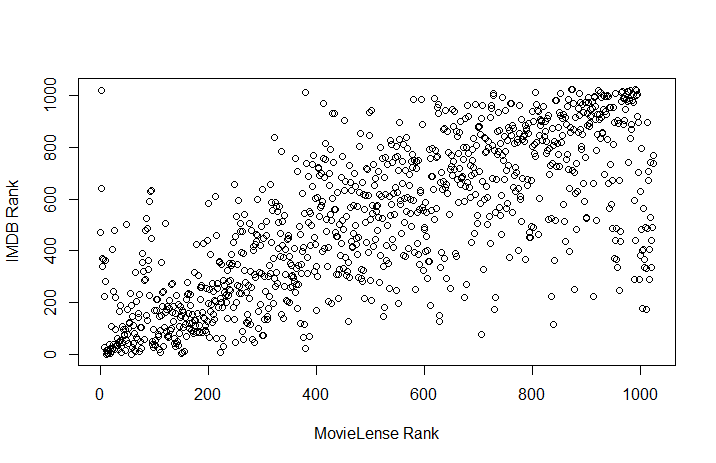
\includegraphics[width=0.7\textwidth]{Q5.png}}
			\label{fig:MovieLense Rank v.s. IMDB Rank}
			\caption{MovieLense Rank v.s. IMDB Rank}
		\end{figure}
		\begin{table}[!htb]
			\centering
			\caption{\textbf{Pearson's Correlation Test Result of MovieLense Rank v.s. IMDB Rank}}
			\begin{tabular}{cc}
				\toprule
				\textbf{Correlation} & \textbf{p-value}\\
				0.7456695 & 2.2e-16\\
				\bottomrule
			\end{tabular}
		\end{table}

		According to the p-value, the correlation between these 2 ranks definitely exists. And the correlation index is 0.75, which tells that the correlation is relatively strong. So it may imply that the two user bases are interchangable.\\
		\section{MovieLense data v.s. IMDB Memento data}
		Repeat \#5, but IMDB data from approximately July 31, 2005. What is the cumulative error from the desired target day of July 31, 2005?\\

		\noindent\textbf{Algorithm:}\\
		\indent1. Use the script from ``Programming Collective Intelligence'' to open the movie data.\\
		\indent2. For each movie, open the URL and get the final URL from HTTP response.\\
		\indent3. Open the timemap of the final URL and get the memento list.\\
		\indent4. Iterate the memento list to get the first memento after 2005-07-31. Try to open this memento to get the rating and voters and save them into \href{https://github.com/zhangboroy/cs532-s17/blob/master/assg07_submission/IMDBmementoRating.csv}{``IMDBmementoRating.csv''}. Otherwise, try next memento.\\
		\indent5. Open \href{https://github.com/zhangboroy/cs532-s17/blob/master/assg07_submission/IMDBmementoRating.csv}{``IMDBmementoRating.csv''} and use the script from ``Programming Collective Intelligence'' to open the MovieLense rating data and transform it.\\
		\indent6. For each movie in \href{https://github.com/zhangboroy/cs532-s17/blob/master/assg07_submission/IMDBmementoRating.csv}{``IMDBmementoRating.csv''}, compute the voters and average rating of users in MovieLense data.\\
		\indent7. Sort the IMDB memento rating data and MovieLense rating data by rating and voters.\\
		\indent8. Replace the IMDB memento rating data and MovieLense rating data with movie ID and rank.\\
		\indent9. For each movie in \href{https://github.com/zhangboroy/cs532-s17/blob/master/assg07_submission/IMDBmementoRating.csv}{``IMDBmementoRating.csv''}, save its ID, MovieLense rank and IMDB memento rank into \href{https://github.com/zhangboroy/cs532-s17/blob/master/assg07_submission/MementoRankContrast.csv}{``MementoRankContrast.csv''}.\\
		\indent10. Open \href{https://github.com/zhangboroy/cs532-s17/blob/master/assg07_submission/MementoRankContrast.csv}{``MementoRankContrast.csv''} in R, plot the scatter and run the Pearson's correlation test.\\

		\noindent\textbf{Source code:}
		\lstinputlisting[language=python, breakatwhitespace=false, label=mementoDownload.py, caption=The content of mementoDownload.py]{mementoDownload.py}
		\lstinputlisting[language=python, breakatwhitespace=false, label=mementoMissingDownload.py, caption=The content of mementoMissingDownload.py]{mementoMissingDownload.py}
		\lstinputlisting[language=python, breakatwhitespace=false, label=Q6.py, caption=The content of Q6.py]{Q6.py}
		\lstinputlisting[language=R, breakatwhitespace=false, label=Q6.R, caption=The content of Q6.R]{Q6.R}

		\noindent\\\textbf{Results:}
		\begin{figure}[!htb]
			\centering 
			\href{https://github.com/zhangboroy/cs532-s17/blob/master/assg07_submission/Q6.png}
			{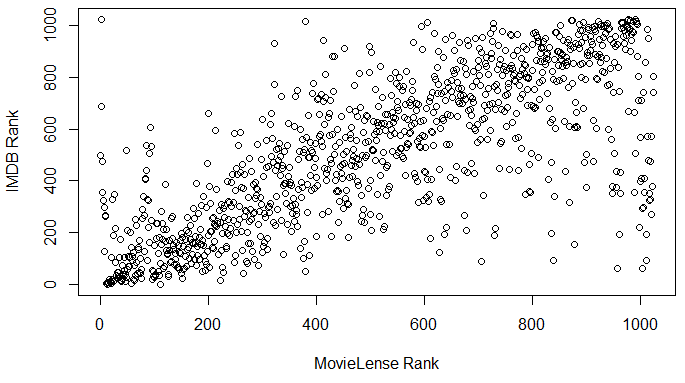
\includegraphics[width=0.7\textwidth]{Q6.png}}
			\label{fig:MovieLense Rank v.s. IMDB memento Rank}
			\caption{MovieLense Rank v.s. IMDB memento Rank}
		\end{figure}
		\begin{table}[!htb]
			\centering
			\caption{\textbf{Pearson's Correlation Test Result of MovieLense Rank v.s. IMDB Memento Rank}}
			\begin{tabular}{cc}
				\toprule
				\textbf{Correlation} & \textbf{p-value}\\
				0.755944 & 2.2e-16\\
				\bottomrule
			\end{tabular}
		\end{table}

		Cumulative Error: see \href{https://github.com/zhangboroy/cs532-s17/blob/master/assg07_submission/cumulativeError.txt}{cumulativeError.txt}\\

		According to the p-value, the correlation between these 2 ranks definitely exists. And the correlation index is 0.76, which tells that the correlation is relatively strong. So it may imply that the two user bases are interchangable.\\
	\end{document}